\documentclass[11pt, notitlepage]{report}

	\usepackage[margin=1in]{geometry}
	\usepackage{amsmath,amsthm,amssymb,amsfonts}
	\usepackage{enumitem}
	\usepackage{systeme}

	\newcommand{\N}{\mathbb{N}}
	\newcommand{\Z}{\mathbb{Z}}
	\newcommand{\R}{\mathbb{R}}
	\newcommand{\A}{\alpha}
	\newcommand{\ora}[1]{\overrightarrow{#1}}
	\newcommand{\Question}[1]{\newpage\section{#1}}
	\usepackage[parfill]{parskip}
	\usepackage{mathtools}
	\newenvironment{solution}{\paragraph{Solution:}}{\hfill}
	\newenvironment{theorem}{\paragraph{Theorem:}}{\hfill}
	\newenvironment{subtheorem}[1]{\paragraph{\small Subtheorem #1:}}{\hfill}
	\newenvironment{definition}{\paragraph{Definition:}}{\hfill}
	\newenvironment{problem}[2][Problem]{\begin{trivlist}
	\item[\hskip \labelsep {\bfseries #1}\hskip \labelsep {\bfseries #2.}]}{\end{trivlist}}
	
	\usepackage{pgfplots}
	\usetikzlibrary{arrows}
	\usetikzlibrary{decorations.markings}
	\usetikzlibrary{datavisualization}
	\usetikzlibrary{datavisualization.formats.functions}
	%\usepackage{pstricks-add}

	\pgfplotsset{every axis/.append style={
	                   axis x line=middle,    % put the x axis in the middle
	                   axis y line=middle,    % put the y axis in the middle
	                   axis line style={<->,color=gray}, % arrows on the axis
	                   xlabel={$x$},          % default put x on x-axis
	                   ylabel={$y$},          % default put y on y-axis
	           }}
	\pgfplotsset{compat=1.15}
	
	\newcommand{\pgraph}[4]{
		\begin{center}
		
		\begin{tikzpicture}
		\begin{axis}[
		   trig format plots=rad,
		   axis equal,
		   grid=both
		]
		\addplot [domain=#3:#4, variable=\t, samples=50, black, decoration={
		   markings,
		   mark=between positions 0.2 and 1 step 4em with {\arrow [scale=1.5]{stealth}}
		   }, postaction=decorate]
		({#1}, {#2});
		
		\end{axis}
		\end{tikzpicture}
		
		\end{center}
	}


   \newcommand{\cgraph}[3]{
	   \begin{center}
	
	   \begin{tikzpicture}
	   \begin{axis}[
	       trig format plots=rad,
	       axis equal,
	       grid=both
	   ]
	   \addplot [domain=#2:#3, variable=\x, samples=50, black, decoration={
	       markings,
	       mark=between positions 0.2 and 1 step 4em with {\arrow [scale=1.5]{stealth}}
	       }, postaction=decorate]
	   {#1};
	
	   \end{axis}
	   \end{tikzpicture}
	
	   \end{center}
	}


	
	\makeatletter
	\newcommand*{\toccontents}{\@starttoc{toc}}
	\makeatother


\begin{document}
   \title{CS70: Homework 3}
   \author{Abhijay Bhatnagar}
   \maketitle
   \toccontents



\setcounter{secnumdepth}{0} %% no numbering

\section{Sundry}

I primarily worked alone, but I talked through some of my proofs with a friend to flesh them out. Received assistance from:

 George Matheos: georgematheos@berkeley.edu
(310) 435-1961.

\newpage
\section{Problem 1: Short Answer: Graphs}

\begin{enumerate}[label=(\alph*)]
\item
Bob removed a degree $3$ node in an $n$-vertex tree, how many connected
components are in the resulting graph?  (An expression that may
contain $n$.)
\begin{solution}
Three. A tree is minimally connected, so removing a degree 3 node creates 3 separate connected components.

\end{solution}
\item
Given an $n$-vertex tree, Bob added 10 edges to it, then Alice removed 
5 edges and the resulting graph has 3 connected components.
How many edges must be removed to remove all cycles
in the resulting graph? (An expression that may contain $n$.)
\begin{solution}
Seven. The addition of any edge in a tree creates a cycle. Bob added 10 edges, creating in the worst case scenario 10 cycles. Alice removed 5 edges, leaving 3 connected components were created, implying that in the worst case scenario 2 of those removed edges were between weakly connected nodes, and three were not, i.e. only three were removed from cycles. In order to guarantee you removed all cycles, you must remove 7.

\end{solution}
\item
True or False: For all $n \geq 3$, the complete graph on $n$ vertices, $K_n$ has more
edges than the $n$-dimensional hypercube. Justify your answer.
\begin{solution}
	False. Consider the counter example, $n=3$. The complete graph $K_3$ has exactly $\frac{3(2)}{2}=3$ edges, while the 3-dimensional hypercube (i.e. a normal cube) has $3\cdot2^{3-1}=12$ edges.
	
\end{solution}
\item
A complete graph with $n$ vertices where $n$ is an odd prime can have all its edges
covered with $x$ Hamiltonian cycles (a Hamiltonian cycle is a cycle where
each vertex appears exactly once). What is the number, $x$,  of
such cycles required to cover the a complete graph? (Answer should be an expression that depends on $n$.)
\begin{solution}
	$\frac{n-1}{2}$. During a hamiltonian cycle, you can travel at most $n$ edges. A complete graph has exactly $\frac{n(n-1)}{2}$ edges, which would require $\frac{n(n-1)}{2} /(n) = \frac{n-1}{2}$ cycles. (This only holds when $\frac{n-1}{2} \in \N \implies n$ is odd.)
	
\end{solution}

\item
Give a set of edge-disjoint Hamiltonian cycles that covers the edges of $K_5$, the complete
graph on $5$ vertices.
(Each path should be a sequence (or list) of edges in $K_5$, where an edge is written as a pair of vertices from the set $\{0, 1, 2, 3, 4\}$ - e.g: $(0, 1), (1, 2)$.)
\begin{solution}
	\{(0,1),(1,2),(2,3),(3,4),(4,0)\},\{(0,2),(2,4),(4,1),(1,3),(3,0)\}
\end{solution}

\end{enumerate}


\Question{Problem 2: Eulerian Tour and Eulerian Walk}

\begin{center}
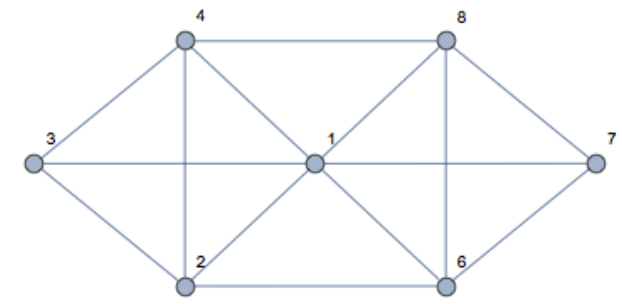
\includegraphics{eulerianquestiongraph}	
\end{center}

\begin{enumerate}[label=(\alph*)]
    \item Is there an Eulerian tour in the graph above?

	\begin{solution}
		Yes: \{(3,4), (4,2), (2,3), (3,1), (1,2), (2,6), (6,1), (1,4), (4,8), (8,1), (1,7), (7,8), (8,6), (6,7)\}
		
	\end{solution}

    \item Is there an Eulerian walk in the graph above?

	\begin{solution}
		No. The graph is not even degreed.
		
	\end{solution}

    \item What is the condition that there is an Eulerian walk in an undirected graph? Briefly justify your answer.
    \begin{solution}
    	An undirected graph contains an Eulerian walk if and only:    	
    	\begin{enumerate}[label=\roman*.)]
    	\item If all edges belong on the same connected component, as you cannot construct a walk that traverses edges on disconnected components.
    	\item There are exactly zero or two odd degreed vertices, as a graph has an even number of odd degreed vertices if any, and every intermediate vertex in an Eulerian walk has to be even degreed. In the case of the two ends, the in-degrees do not necessarily have to equal the out-degrees in a walk, therefore they can be odd-degreed.
    	\end{enumerate}
    \end{solution}
\end{enumerate}



\Question{Problem 3: Bipartite Graph}
A bipartite graph consists of $2$ disjoint sets of vertices (say $L$ and $R$), such that no $2$ vertices in the same set have an edge between them. 
% For example, if we had a bipartite graph that consists of vertices $\{1, 2, 3, 4\}$, such that set A = $\{1, 2\}$ and B = $\{3, 4\}$, there cannot exist an edge between $1$ and $2$, and similarly there cannot exist an edge between $3$ and $4$. \\
For example, here is a bipartite graph (with $L=\{\hbox{{\color{green}{green}} vertices}\}$ and $R =\{\hbox{{\color{red}{red}} vertices}\}$),  and a non-bipartite graph.

	\begin{figure}[hpb]
\begin{minipage}{0.49\textwidth}
	\centering
	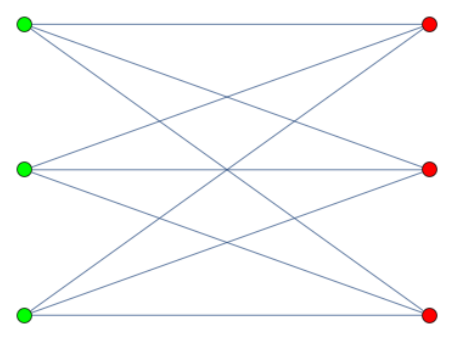
\includegraphics[scale=.6]{k_3_3}
\end{minipage}
\begin{minipage}{0.49\textwidth}
	\centering
	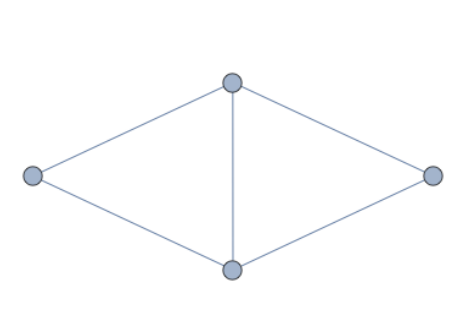
\includegraphics[scale=.3]{non-bipartite}
\end{minipage}
\caption{A bipartite graph (left) and a non-bipartite graph (right).}
	\label{fig:bipartite}
	\end{figure}

Prove that a graph is bipartite if and only if it has no tours of odd length.
\vskip 0.5in
\begin{solution}
To prove the previous theorem, we must prove both a graph is bipartite only if it has no tours of odd-length, and that a graph with no tours of odd length  

\begin{subtheorem}{1}
	A graph is is bipartite only if it has no tours of odd-length.
	\begin{proof}
		We proceed by contradiction. Assume a bipartite graph has a tour $v \rightarrow v$ of odd-length. As a bipartite graph has two disjoint sets of vertices, every walk of length one must traverse between a vertex in one set to a vertex in the other, which implies all walks of an odd length must end in the opposite set of the origin, which in turn implies $v \rightarrow v$ must end in the opposite set of the origin. As $v \rightarrow v$ is a tour, this is a contradiction, as desired.	
	\end{proof}
\end{subtheorem}
\begin{subtheorem}{2}
	A graph that has no tours of odd-length is bipartite.
	\begin{proof}
		Assume a connected graph has no tours of odd-length. For any point $v$, consider all points $v_{even}$ s.t. the distance from $v_{even}\rightarrow v$ is even. Similarly, consider all points $v_{odd}$ s.t. the distance from $v_{odd}\rightarrow v$ is odd.   If there existed an edge within two vertices in $v_{even}$, that would imply there exists a tour to $v$ of odd length. Similarly, If there existed an edge within two vertices in $v_{odd}$, there would be the same implication. Since the graph has no tours odd-length, there must be no edges between vertices within the same set. Since $\forall v,v\in v_{even}$, we have 2 disjoint sets of vertices s.t. no 2 vertices in the same set have a connecting edge, which is the desired result.
	\end{proof}
\end{subtheorem}
\end{solution}
\Question{Problem 4: Hypercubes}
The vertex set of the $n$-dimensional hypercube $G=(V,E)$ is given by $V=\{0,1\}^n$ (recall that $\{0,1\}^n$ denotes the set of all $n$-bit strings). There is an edge between two vertices $x$ and $y$ if and only if $x$ and $y$ differ in exactly one bit position. These problems will help you understand hypercubes.

\begin{enumerate}[label=(\alph*)]
\item Draw 1-, 2-, and 3-dimensional hypercubes and label the vertices using the corresponding bit strings.

\begin{solution}\

1-dimensional: 
\begin{center}
  
\begin{tikzpicture}
  [scale=.8,auto=left,every node/.style={circle,fill=black!20}]
  \node[label=left:{\small 0}] (n1) at (0,0)  {};
  \node[label=right:{\small 1}] (n2) at (2,0)  {};

  \foreach \from/\to in {n1/n2}
    \draw (\from) -- (\to);
\end{tikzpicture}
\end{center} \vskip .3in
2-dimensional: 
\begin{center}
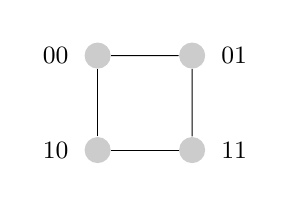
\begin{tikzpicture}
  [scale=.6,auto=left,every node/.style={circle,fill=black!20}]
  \node[label=left: {\small 10}] (n1) at (0,0)  {};
  \node[label=left: {\small 00}] (n2) at (0,2)  {};
  \node[label=right:{\small 01}] (n3) at (2,2)  {};
  \node[label=right:{\small 11}] (n4) at (2,0)  {};

  \foreach \from/\to in {n1/n2,n2/n3,n3/n4,n4/n1}
    \draw (\from) -- (\to);
\end{tikzpicture}
\end{center}
3-dimensional: 
\begin{center}
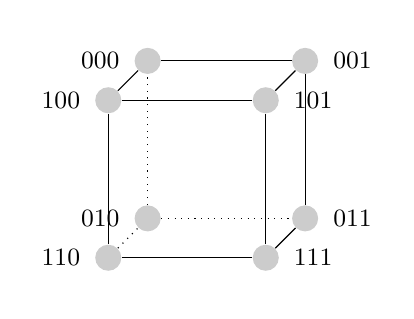
\begin{tikzpicture}
  [scale=.5,auto=left,every node/.style={circle,fill=black!20}]
  \node (n1)[label=left: {\small 110}] at (0,0)  {};
  \node (n2)[label=left: {\small 100}] at (0,4)  {};
  \node (n3)[label=right:{\small 101}] at (4,4)  {};
  \node (n4)[label=right:{\small 111}] at (4,0)  {};

  \node (n5)[label=left: {\small 010}] at (1,1)  {};
  \node (n6)[label=left: {\small 000}] at (1,5)  {};
  \node (n7)[label=right:{\small 001}] at (5,5)  {};
  \node (n8)[label=right:{\small 011}] at (5,1)  {};

  \foreach \from/\to in {n1/n2,n2/n3,n3/n4,n4/n1,n2/n6,n3/n7,n4/n8,n8/n7,n6/n7}
    \draw (\from) -- (\to);
  \foreach \from/\to in {n1/n5,n5/n8,n5/n6}
    \draw [dotted] (\from) -- (\to);
\end{tikzpicture}
\end{center}
\end{solution}
\item Show that for any $n\ge 1$, the $n$-dimensional hypercube is \emph{bipartite}: the vertices can be partitioned into two groups so that every edge goes between the two groups.
\begin{solution}
	\begin{proof}
		By definition, in a hypercube $x$ and $y$ are connected by edge $\{x,y\}$ if and only if $x$ and $y$ differ in exactly one bit position. This implies that vertices of an even $n$-bit string are only connected to vertices of an odd $n$-bit string.  Therefore, a hypercube can be partitioned into two groups of disjoint vertices: 
		
		\-\hspace{2cm}$G_1$ = all points $x : x= x_1,x_2,...,x_n \land 2|\sum{x_1,x_2,...,x_n}$, and 
		
		\-\hspace{2cm}$G_2$ = all points $y : y=y_1,y_2,...,y_n \land 2\nmid \sum{y_1,y_2,...,y_n}$, 
		
		which is the desired result.
	\end{proof}
\end{solution}
\end{enumerate}
\Question {Problem 5: Triangulated Planar Graph}
In this problem you will prove that every triangulated planar graph (every face has 3 sides; that is, every face has three edges bordering it, including the unbounded face)
contains either (1) a vertex of degree 1, 2, 3, 4, (2) two degree 5 vertices 
which are adjacent, or (3) a degree 5 and a degree 6 vertices which are 
adjacent. Justify your answers.

\begin{enumerate}[label=(\alph*)]
\item Place a ``charge'' on each vertex $v$ of value $6-\operatorname{degree}(v)$. What is
the sum of the charges on all the vertices?
(\textit{Hint}: Use Euler's formula and the fact that the planar graph is
triangulated.)

\begin{solution} 12.
	Given planar graph is triangulated, we know each face is bordered by three edges and each edge must border exactly two faces,  $f=\frac{2e}{3}$. Inserting that into $v+f=e+2$, we can then find $e=3v-6$. Since each edge increases the degree of two vertices, we can consider the `average` degree on a vertex $= \frac{2e}{v}$. Similarly, we can consider the $\text{`average` charge} = 6-\text{average degree}$. From there:
	\begin{align*}
		\sum{charge(v)}&=\text{(average charge)}\cdot v \\
					   &=[6-\text{(average degree)}]\cdot v \\
					   &=[6-\frac{2(3v-6)}{v}]\cdot v \\
					   &=6v-6v+12 \\
					   &=12 \\
	\end{align*}
\end{solution}

\item What is the charge of a degree $5$ vertex and of a degree $6$ vertex?
\begin{solution}
	Charge(degree 5 vertex) = 1. Charge(degree 6 vertex) = 2.
\end{solution}
\item Suppose now that we shift $1/5$ of the charge of a degree $5$ vertex to each of its neighbors that has a negative charge.  (We refer to this as ``discharging'' the degree $5$ vertex.)  Conclude the proof under the assumption that, after discharging all degree $5$ vertices, there is a degree $5$ vertex with positive remaining charge.
%Move $1/5$ charge from each degree $5$ vertex to each of its negatively charged 
%neighbors. Conclude the proof in the case where there is a degree $5$
%vertex with positive remaining charge. 
\begin{solution}
	If there exists a degree 5 vertex with positive remaining charge, that must imply at least one neighbor that had nonnegative charge, i.e. it must have a degree $\leq 6$. If that neighbor had a degree $\leq 4$, case (1) holds. If it had a degree $= 5$, case (2) holds. Otherwise, if it had a degree $= 6$, case (3) holds.
\end{solution}
\newpage
\item If no degree $5$ vertices have positive charge after discharging the degree $5$ vertices, 
does there exist any vertex with positive charge after discharging?
If there is such a vertex, what are the possible degrees of that vertex?
\begin{solution}
	If all degree 5 vertices have completely discharged, all of their neighbors must have a negative charge. In order for there to exist a vertex with degree $n>6$ such that its charge afterwards is positive, its original charge plus discharges must be positive, i.e.  $\exists n\in \N: n>6 \land 6-n+\frac{n}{5}>0  \implies 6<n<\frac{15}{2}.$ This is possible when $n=7$. Therefore, a vertex with degree 7 would be a possible degree. (Additionally, if there were any vertices of degrees $n\leq 4$ connected to the other edges of the negatively charged vertices, those would have positive final charges, so those would be possible degrees of vertices existing in the graph as well, but those are trivial cases.)
\end{solution}
\item 
Suppose there exists a degree $7$ vertex with positive charge after discharging the degree $5$ vertices.
How many neighbors of degree $5$ might it have?
\begin{solution}
	At least 6. A degree 7 vertex has a charge of $-1$, so it needs at least 6 increments of $1/5$ to become positive.
\end{solution}

\item Continuing from item (e). Since the graph is triangulated, 
  are two of these degree $5$ vertices adjacent?
\begin{solution}
	Since the graph is triangulated, there must exist edges connecting every adjacent pair of adjacent edges off of the degree 7 vertex. Since at least 6 of edges of the degree 7 vertex are degree 5 vertices, at least two of them are connected by an edge, which implies the are adjacent.
\end{solution}

\item Finish the proof from the facts you obtained from the previous
  parts.
  
  
  \begin{proof}
  	  Assume G is a triangular planar graph. Since we know the charge on the planar graph has to equal 12, we know the vertex cannot solely be composed of vertices of degree $n\geq 6$, as the sum of its charges will be $\leq 0$. Therefore there must exist some vertex with degree $n\leq 5$.
  
  If there exists in the graph a vertex of degree $n\leq 4$, case (1) immediately holds. This is trivial.
  
  If there exists in the graph a vertex of degree $n=5$, we can 'discharge' it and proceed to look at the two cases:
  \begin{enumerate}[label=\roman*.)]
  	\item There exists at least one degree 5 with a remaining positive charge: 

In this case, part (c) holds true, i.e. the degree 5 vertex must have a neighbor of degree $n \leq 6$. If that neighbor had a degree $n \leq 4$, case (1) holds. If it had a degree $n = 5$, case (2) holds. Otherwise, if it had a degree $n = 6$, case (3) holds.
  	\item All degree 5 vertices are discharged: 

  	In this case, parts (d), (e), and (f) hold true, i.e. there must exist adjacent two degree 5 vertices and case (2) holds. 
  \end{enumerate}
  In all cases, either case (1), (2), or (3) must be true, which is the desired result.
  \end{proof}
  



\end{enumerate}





\end{document}
